% !TeX spellcheck = en_GB 
\section{Introduction}
Multi-material FDM 3D printers unlock a plethora of applications through combining the unique material properties of various materials.
However, depending on the combination of materials the adhesion between the materials can be negligibly weak.
While only a small number of all possible 3D printing material combinations may exhibit any incompatibility issues,
it is often precisely those incompatible combinations where the different chemical make-up produces interesting applications.
For example, polypropylene (PP) is semi-flexible and fatigue-resistant, but has a very weak chemical bond to typical rigid filaments such as polylactic acid (PLA).
In such cases it is necessary to rely on mechanical interlocking to prevent the materials from breaking apart from each other.



\begin{figure}
	\centering
	\setlength{\figheight}{.45\columnwidth}\centering
	\begin{subfigure}[B]{.25\columnwidth}
		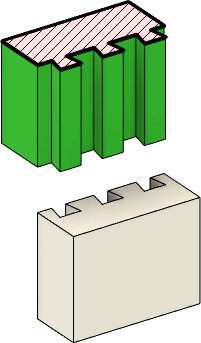
\includegraphics[height=\figheight]{sources/method/basic_2d_interlock.jpg}
		\caption{A 2D dovetail interlock}
		\label{fig:basic_2d_interlock}
	\end{subfigure}
	\begin{subfigure}[B]{.36\columnwidth}\centering
		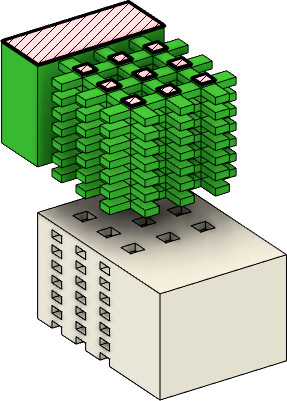
\includegraphics[height=\figheight]{sources/method/discontinuous_lattice.jpg}
		\caption{Cubic lattice with disconnected islands}
		\label{fig:discontinuous_lattice}
	\end{subfigure}
	\begin{subfigure}[B]{.36\columnwidth}\centering
		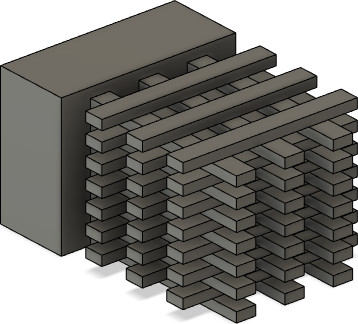
\includegraphics[height=\figheight]{sources/method/basic_lattice.jpg}
		\caption{The ITIM lattice with long continuous paths}
		\label{fig:basic_structure_single_mat}
	\end{subfigure}
	\caption{Interlocking principles; exploded view with a section cut at the top layer. The dovetail can be disassembled by translation; the cubic lattice causes highly discontinuous extrusion on some layers; the proposed ITIM lattice solves these problems.}
	\label{fig:basic_structure}
\end{figure}






A common type of interlocking can be found in jigsaw puzzles.
The pieces interlock and stay connected because of the material stiffness.
However, the interlock can be broken in plane by deformation of the pieces.
Out of plane the pieces can be disassembled easily.
See \cref{fig:basic_2d_interlock}.

In order to overcome these limitations, we invoke the mathematical study of topology.
Topology is the study of properties of geometric shapes which are preserved under continuous deformations, such as stretching, twisting and bending.
The property of \emph{genus} counts how many holes a shape has;
a ball has a genus of 0, a doughnut has a genus of 1 and pants have a genus of 2.

If the holes in the geometry of one material are filled with the other material we achieve a new type of interlocking, which we call \emph{topological interlocking}.
Doughnuts can be imagined to be chained together to form the geometry of a chain.
The only way to disassemble a chain is by breaking one of the links.
%They cannot be broken by deformation alone, because links of a chain have a topology of genus 1.
An interlocking geometry with a high genus topology means that the interlock is preserved under deformations of the two materials.
This interlocking principle is robust especially when flexible and deformable materials are concerned.

For the application of dual material FDM we propose a high genus topologically interlocking structure where all voids in the one material are filled with the other material and vice versa.
However, most high genus geometries would introduce discontinuities in the extrusion process when sliced into layers for 3D printing, as each slice would contain disconnected islands.
See \cref{fig:discontinuous_lattice}.
Such discontinuities lead to defects, which influence the accuracy and the mechanical properties of the resulting part.
Moreover, depositing small disconnected islands of one material on top of a chemically incompatible material cannot reliably be performed because of the weak bonding.
We therefore have to generate interlocking geometry for which the layers consist of long continuously connected areas for both materials.

Intuitively it seems impossible to generate high genus interlocking geometry while enforcing continuous extrusion for both materials;
if the one material leaves a hole in a layer then filling that hole with the other material will cause it to be disconnected from the other regions of the second material.
The ITIM lattice consists of long horizontal beams which ensure continuous extrusion, which alternate in orientation along the Z axis in order to connect all beams together, thereby ensuring the high genus of the topology.
The holes are then all aligned horizontally in between the layers, so that they never result in disconnected islands.
See \cref{fig:basic_structure_single_mat}.


Our contributions are as follows:
\begin{itemize}
	\item A theoretical upper bound to the tensile strength of any interlocking structure.
	\item An interlaced topologically interlocking microstructure (ITIM) which satisfies the extrusion continuity constraint.
	\item Two variations of the ITIM lattice optimized for tensile forces.
	\item Analytical models for estimating tensile properties and for optimizing the design parameters of the interlocking structures.
	\item Numerical and experimental validation.
\end{itemize}






